
%%%%%%%%%%%%%%%%%%%%%%%%%%%%%%%%%%%%%%%%%%%%%%%%%%%%%%%%%%%%%%%%%%%%%%%%%
%           Capítulo 3: Mapeo de Hénon
%%%%%%%%%%%%%%%%%%%%%%%%%%%%%%%%%%%%%%%%%%%%%%%%%%%%%%%%%%%%%%%%%%%%%%%%%
\chapter{Ejemplos de aplicación del método}
%\label{SeccionEstandar}\section{Mapeo estándar}

Utilizando el método ya programado se hicieron diferentes cálculos para encontrar algunas \'orbitas peri\'odicas en el mapeo est\'andar, que se muestran en la figura \ref{orbitasperiodicasestandarv}. Todas las \'orbitas que aparecen fueron calculadas n\'umeros de tipo \textrm{Float64} y presentan un error menor al $1\times10^{-15}$.
\begin{figure}[H]
	\centering
	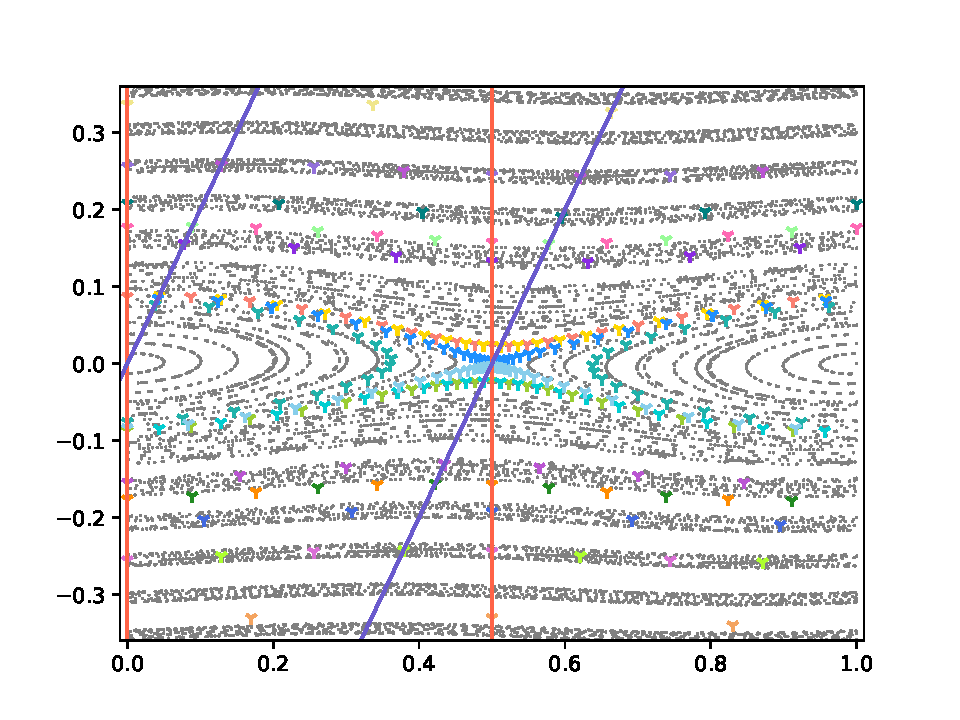
\includegraphics[scale= 0.7]{EstandarOP07}
	\label{orbitasperiodicasestandarv}
	\caption{Espacio fase del mapeo est\'andar, con $\kappa = 0.07$, junto con varias \'orbitas peri\'odicas. Las lineas rojas y azul representan los conjuntos invariantes $\mathbb{J}_{0},\mathbb{J}_{1}$}.
\end{figure}
\begin{figure}[H]
	\centering
	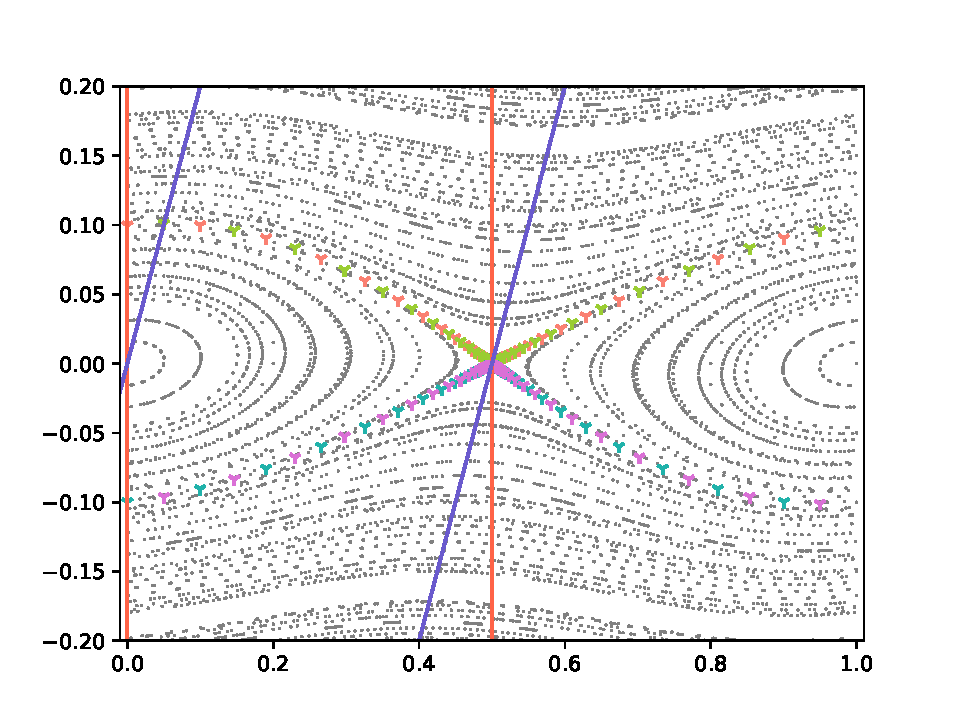
\includegraphics[scale= 0.7]{EstandarOP1-40.pdf}
	\label{orbitasp40estandar}
	\caption{Espacio fase del mapeo est\'andar, con $\kappa = 0.07$, con 4  \'orbitas de periodo 40. Las lineas rojas y azul representan los conjuntos invariantes $\mathbb{J}_{0},\mathbb{J}_{1}$}. 
\end{figure}

Para caclular las \'orbitas se requiere una semilla para iniciar el m\'etodo de Newton, esta semilla se calcul\'o primero calculando las \'orbitas peri\'odicas del mapeo cuando el valor del par\'ametro es $\kappa=0.0$ y el sistema es completamente integrable. \\ 

Otro mapeo con el que se trabaj\'o fue el mapeo cuadr\'atico que es una mapeo que preserva \'area y donde $a,b$ son n\'umeros reales. El mapeo es integrable cuando $b=0$.
\begin{equation}
	M_{a,b}(x_{n},y_{n}) = \left(
	\begin{array}{c}
	x_{n}+a(1-y_{n+1}^{2})\\
	y_{n}-b\sin(2\pi x_{n})
	\end{array}
	\right)
	\label{mapeocuadratico}
\end{equation}
Sus correspondientes involuciones son.
\begin{equation}
	\mathbf{I}_{0}
	\left(\begin{array}{c}
		x\\
		y
	\end{array}
	\right) = 
	\left(-x\\
	y-b\sin(2\pi x)
	\right)
	\label{involucioncuadratico0}
\end{equation}
\begin{equation}
	\mathbf{I}_{1}
	\left(\begin{array}{c}
		x\\
		y
	\end{array}
	\right) = 
	\left(-x+ a(1-y^{2})\\
	y
	\right)
	\label{involucioncuadratico1}
\end{equation}

Mientras que sus conjuntos invariantes asociados son
\begin{equation}
	\mathbb{J}_{0} = \{ (x,y) | x=0 ,x=1/2\}
	\label{conjunto invariante cuadratico 0}
\end{equation}
\begin{equation}	
	\mathbb{J}_{1} = \{ (x,y)| x= a(1-y^{2})/2, x = a(1-y^{2})/2+1/2
		\}
	\label{conjunto invariante cuadratico 1}
\end{equation}
Utilizando el m\'etodo implementado de la misma manera que se utiliz\'o para el mapeo est\'andar es posible obtener \'orbitas peri\'odicas de diferentes periodos usando semillas adecuadas. Un ejemplo de algunas \'orbitas se muestra en la figura \ref{grafmapeocuadratico1}. \\

\begin{figure}
	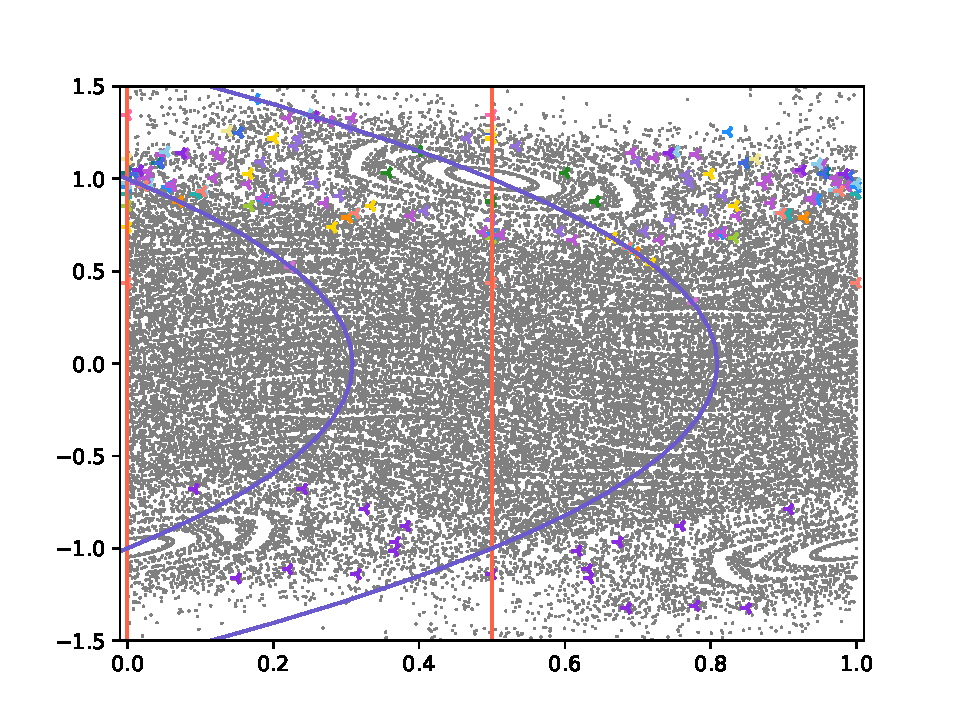
\includegraphics[scale=0.7]{MapeoCuadraDifP}
	\label{grafmapeocuadratico1}
	\caption{Espacio fase y algunas \'orbitas peri\'odicas del mapeo \eqref{mapeocuadratico} con $ a = 0.618, b=0.2$. Las curvas de color rojo y azul corresponden a los conjuntos $\mathbb{J}_{0}, \mathbb{J}_{1}$.} 
\end{figure}
\begin{figure}
	\centering
	\includegraphics[scale=0.6]{MApeoCP4A}
	\caption{\'Orbita de periodo 4 en el mapeo \eqref{mapeocuadratico} con $a = 0.2625, b = 0.44$.}
	\label{grafmapeocuadraper4}
\end{figure}
Es posible dentro del programa implementado cambiar el m\'etodo para encontrar las ra\'ices dentro del m\'etodo. Sin embargo es mejor encontrar la forma de obetener ra\'ices que se aproximen a un punto de la \'orbita  ya que eso garantiza la convergencia del m\'etodo usando los m\'etodos de soluci\'on de ra\'ices m\'as simples. Tambi\'en se implement\'o una extensi\'on del m\'etodo para aritm\'etica de presici\'on extendida. En presici\'on extendida se utilizan n\'umeros de presici\'on arbitraria la cual trabaja con 256 bits predefinida. \\

Algo interesante de analizar con est\'a herramienta es la din\'amica de las \'orbitas peri\'odicas con forme se mueven los par\'ametros. En el caso del mapeo \eqref{mapeocuadratico} se muestra en la figura  \ref{grafmapeocuadraper4variable} c\'omo la \'orbita de periodo 4 se va modificando al variar el par\'ametro $b$ y dejando fijo $a=0.618$.

\begin{figure}
	\centering
	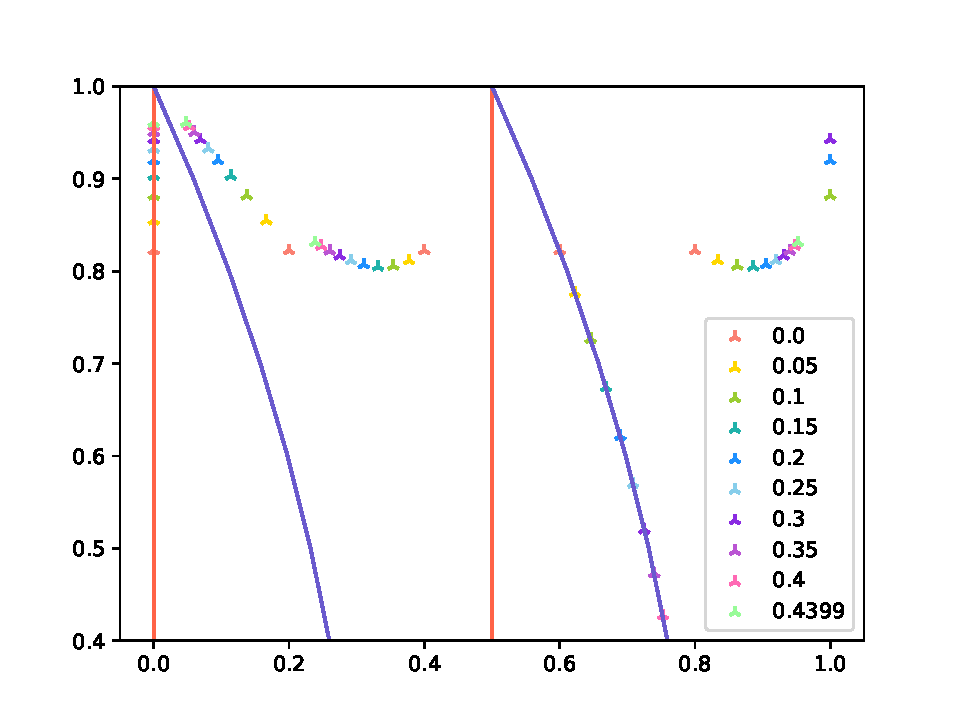
\includegraphics[scale=0.7]{MapeoCuadraP5b}
	\caption{Din\'amica de una \'orbita de periodo 4 del mapeo \eqref{mapeocuadratico} con valores $a=0.618$ fija y $b$ variable. Las curvas rojas y azules corresponden a los conjuntos invariantes $\mathbb{J}_{0}, \mathbb{J}_{1}$. }
	\label{grafmapeocuadraper4variable}
\end{figure}

\section{\'Orbitas peri\'odicas hiperb\'olicas y sus variedades.}
Una vez que se tienen algunas \'orbitas peri\'odicas es posible determinar cu\'ales de ellas son hiperb\'olicas. Seleccionando las que cumplan ser hiprb\'olicas es posible ahora aplicar el m\'etodo de parametrizaci\'on para las variedades asociadas a la \'orbita. \\

En el caso del mapeo est\'andar es bien conocido que existe una \'orbita hiperb\'olica de periodo 2 que persiste para ciertos valores del par\'ametro $\kappa$. Usando diferentes valores del par\'ametro se calcularon las parametrizaciones de las variedades asociadas usando polinomios de orden $70$ evaluados en el intervalo $t=[-0.2,0.2]$. La figura \ref{estandarvariedadesperiodo2} muestra las variedades en el espacio fase asociadas a la \'rbita hiperb\'olica de periodo dos para diferentes valores de $\kappa$. Como s epuede observar mientras el valor de $\kappa$ aumenta las variedades se van abriendo dejando mayor espacio a la din\'amica de la \'orbita el\'iptica de periodo dos. \\



\begin{figure}
	\centering
	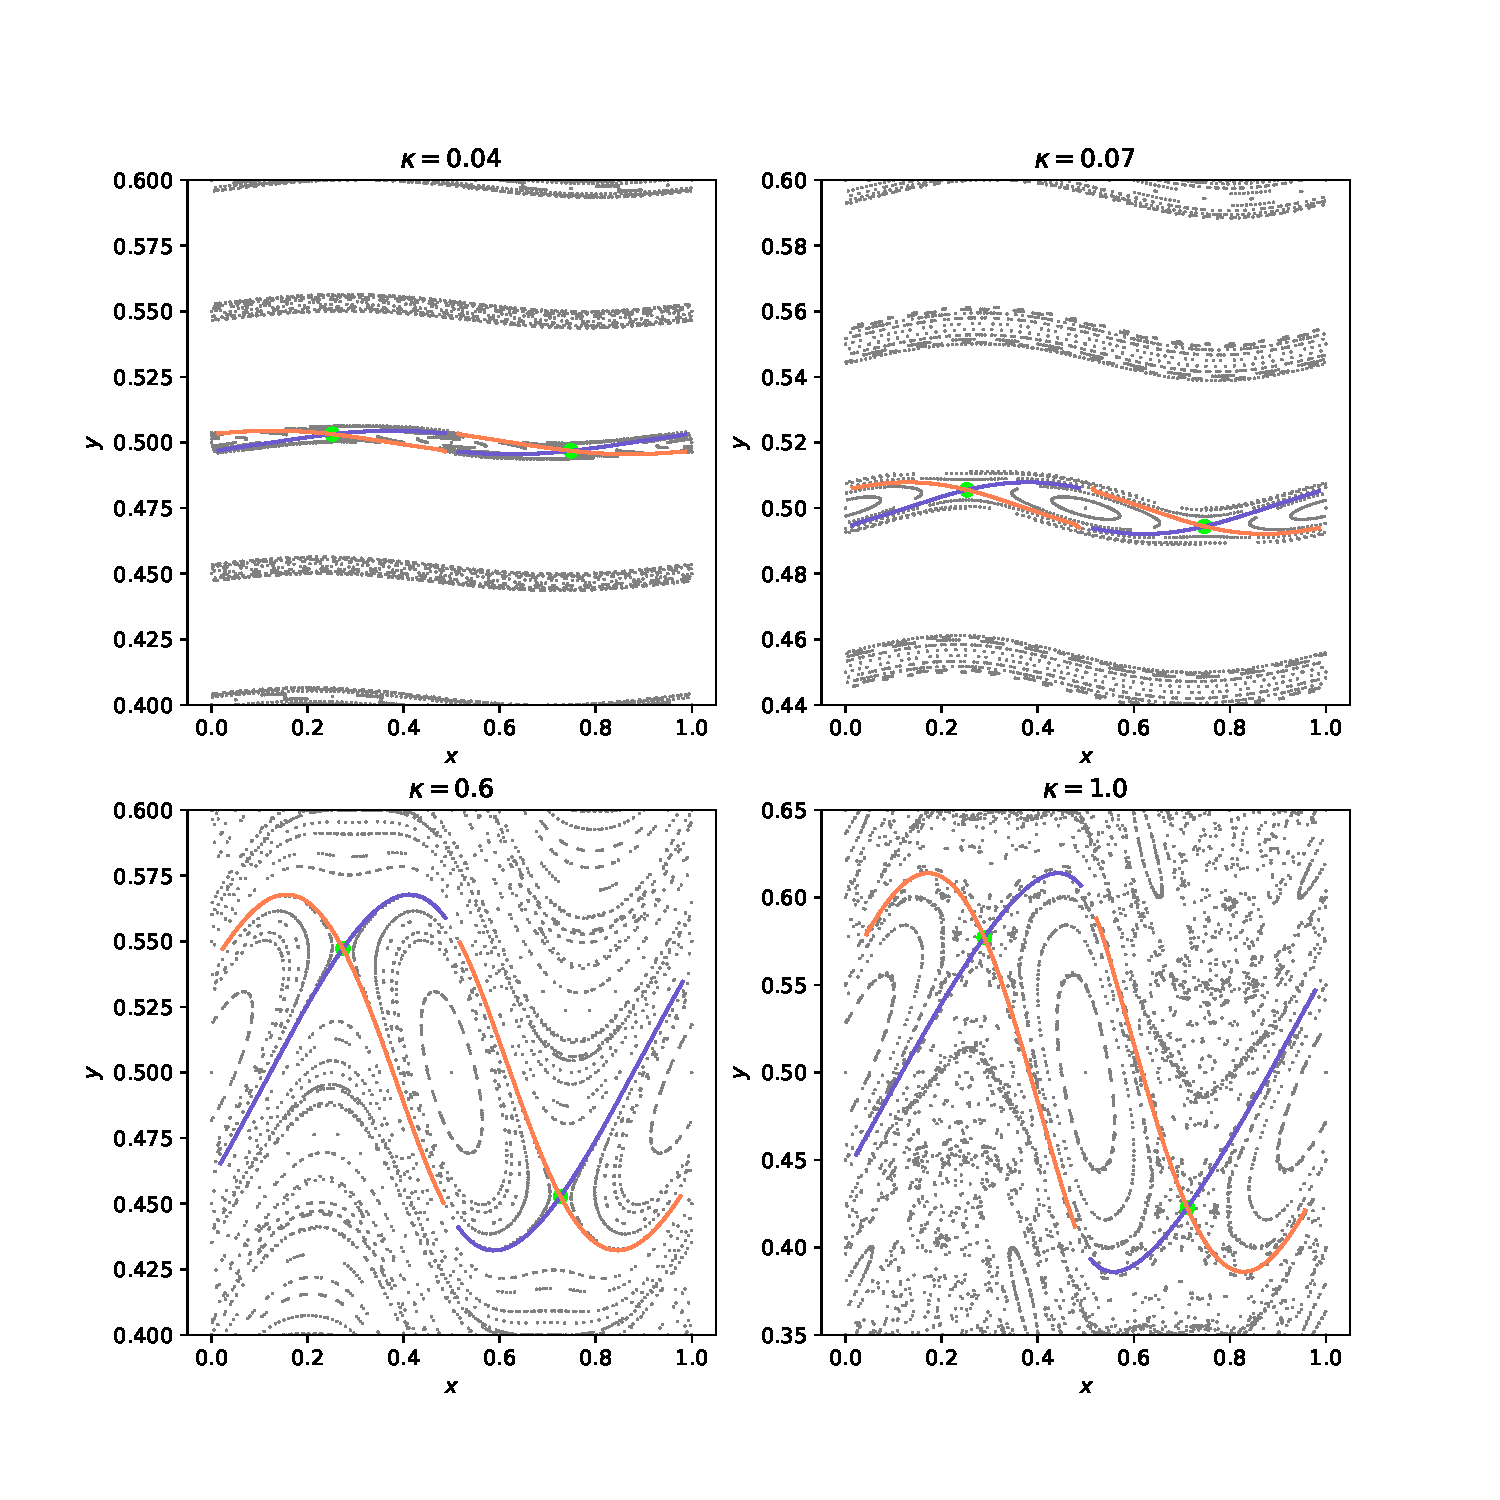
\includegraphics[scale=0.6]{variedadesestandarperiodo2}
	\caption{Variedades invariantes asociadas a la \'orbita de periodo dos en el mapeo est\'andar con diferentes valores de $\kappa$.}
	\label{estandarvariedadesperiodo2}
\end{figure}
\begin{figure}
	\centering
	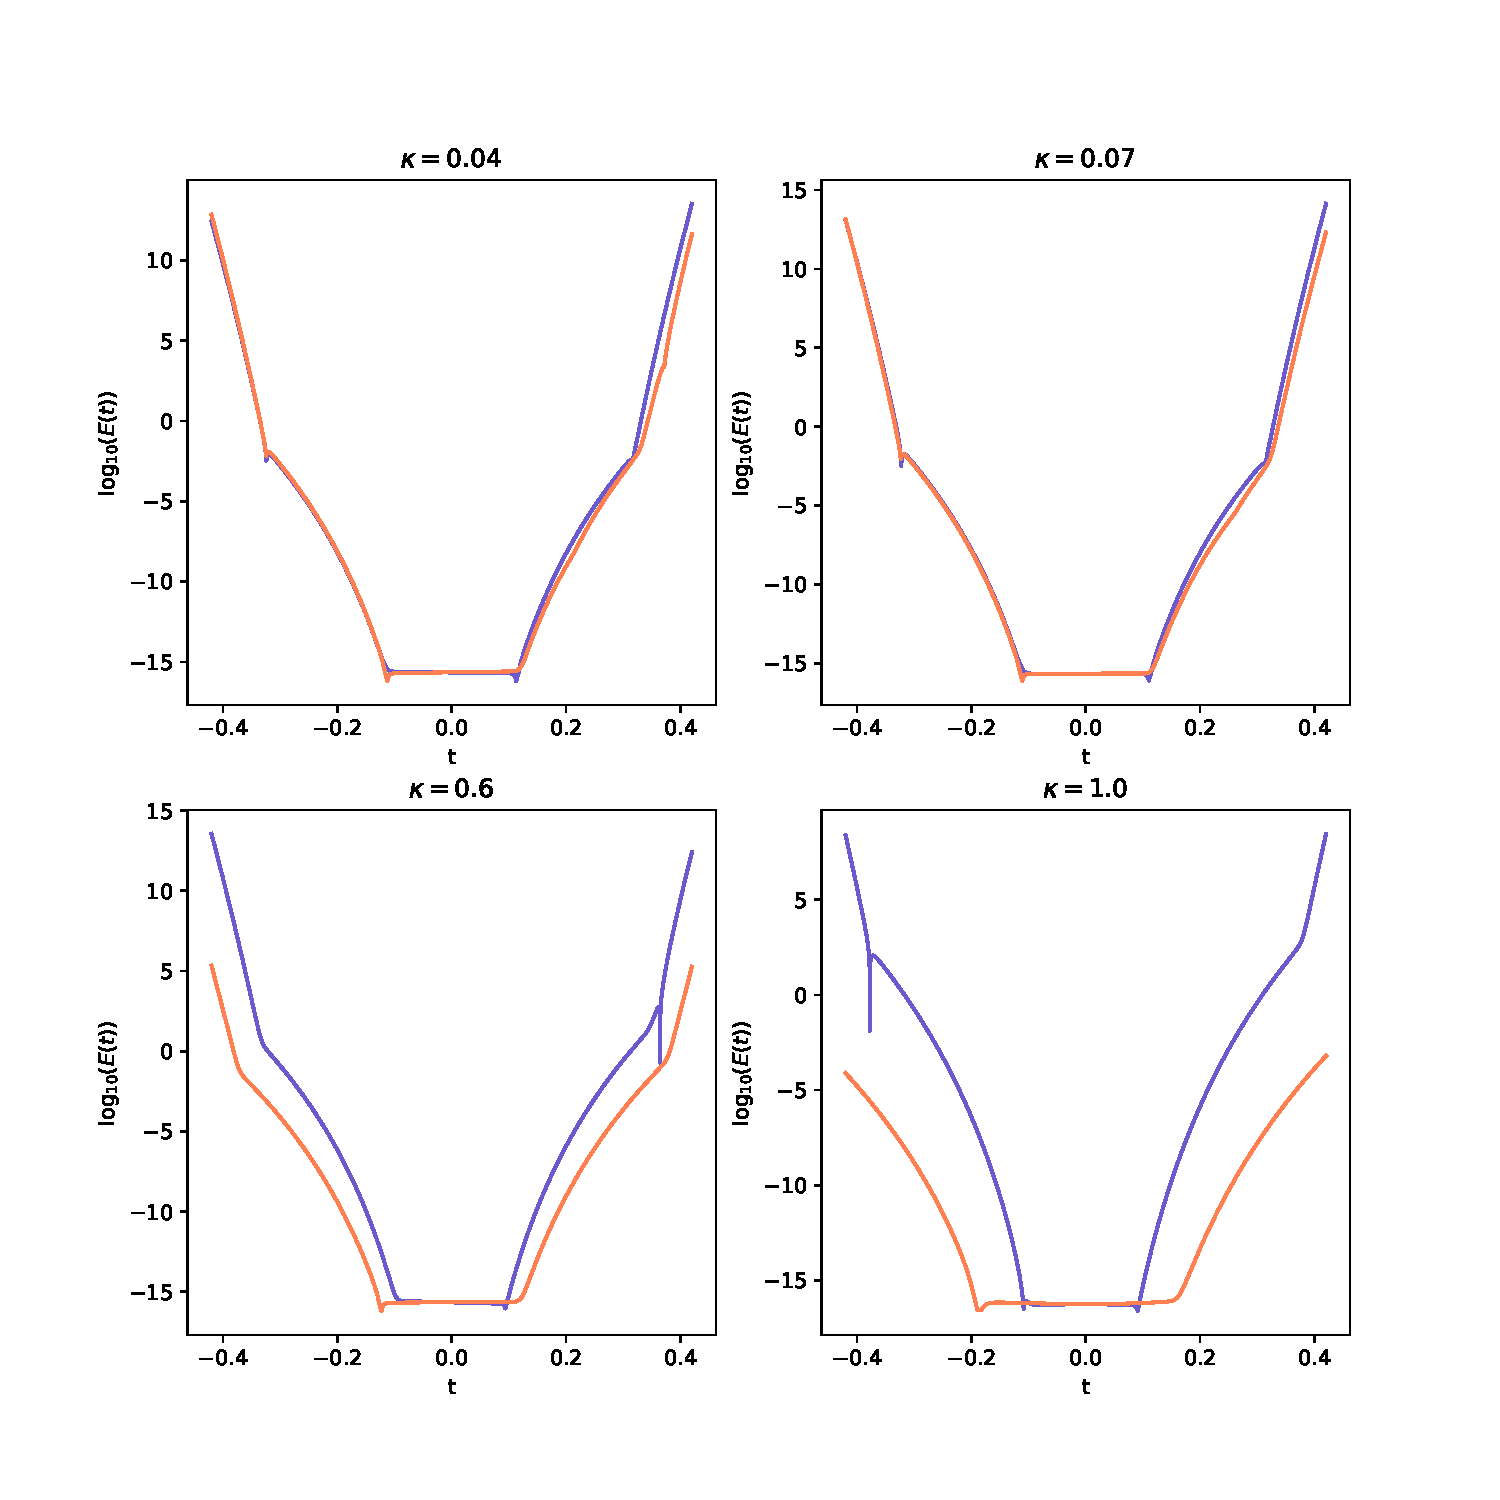
\includegraphics[scale=0.7]{erroresvariedadesestandarperiodo2}
	\caption{Errores asociados al c\'alculo de las variedades invariantes que aparecen en la figura \ref{estandarvariedadesperiodo2}.}
	\label{erroresvariedadesestandarperiodo2}
\end{figure}
Variando el valor de $\kappa$ entre $0.1$ y $1.1$ y calculando las \'orbitas hiperb\'olicas de periodo dos y sus respectivas variedades se obtuvo la figura  \ref{variedadesestandarkappasv} donde se muestra como la \'orbita de periodo dos se va deformando as\'i como las variedades. De cada punto marcado en color verde surge una variedad estable (verde) y una variedad inestable (naranja), se puede notar como la variedad estable se convierte en la inestable del punto siguiente en la \'orbita. 
\begin{figure}
	\centering
	\includegraphics[scale=0.7]{variedadesestandarkappas}
	\caption{Comportamiento de las variedades invariantes asociadas a la \'orbita de periodo dos en el mapeo est\'andar al variar $\kappa$ entre $[0.1,1.1]$.}
	\label{variedadesestandarkappasv}
\end{figure}
\begin{center}
\begin{tabular}{|c|c|}
		\hline
		$\kappa$&  Error  \\
		\hline
		$0.01$ &  $2.220446049250313e-16$\\
		\hline
		$0.02$& $0.0$ \\
		\hline
		$0.03$	& $2.220446049250313e-16$  \\
		\hline
		$0.04$&  $2.220446049250313e-16$\\
		\hline
		$0.05$&  $2.220446049250313e-16$\\
		\hline
		$0.06$&  $2.220446049250313e-16$\\
		\hline
		$0.07$&  $2.220446049250313e-16$\\
		\hline
		$0.08$& $0.0$  \\
		\hline
		$0.09$& $0.0$  \\
		\hline
		$0.1$& $0.0$  \\
		\hline
		$0.2$&$3.3306690738754696e-16$  \\
		\hline
		$0.3$& $2.220446049250313e-16$ \\
		\hline
		$0.4$&$2.220446049250313e-16$  \\
		\hline
		$0.5$&$2.220446049250313e-16$  \\
		\hline
		$0.6$& $4.440892098500626e-16$ \\
		\hline
		$0.7$& $0.0$  \\
		\hline
		$0.8$& $0.0$ \\
		\hline
		$0.9$& $4.440892098500626e-16$   \\
		\hline
		$1.0$& $4.440892098500626e-16$  \\
		\hline
		$1.1$& $4.440892098500626e-16$  \\
		\hline
\end{tabular}
\end{center}
\begin{figure}
	\centering
	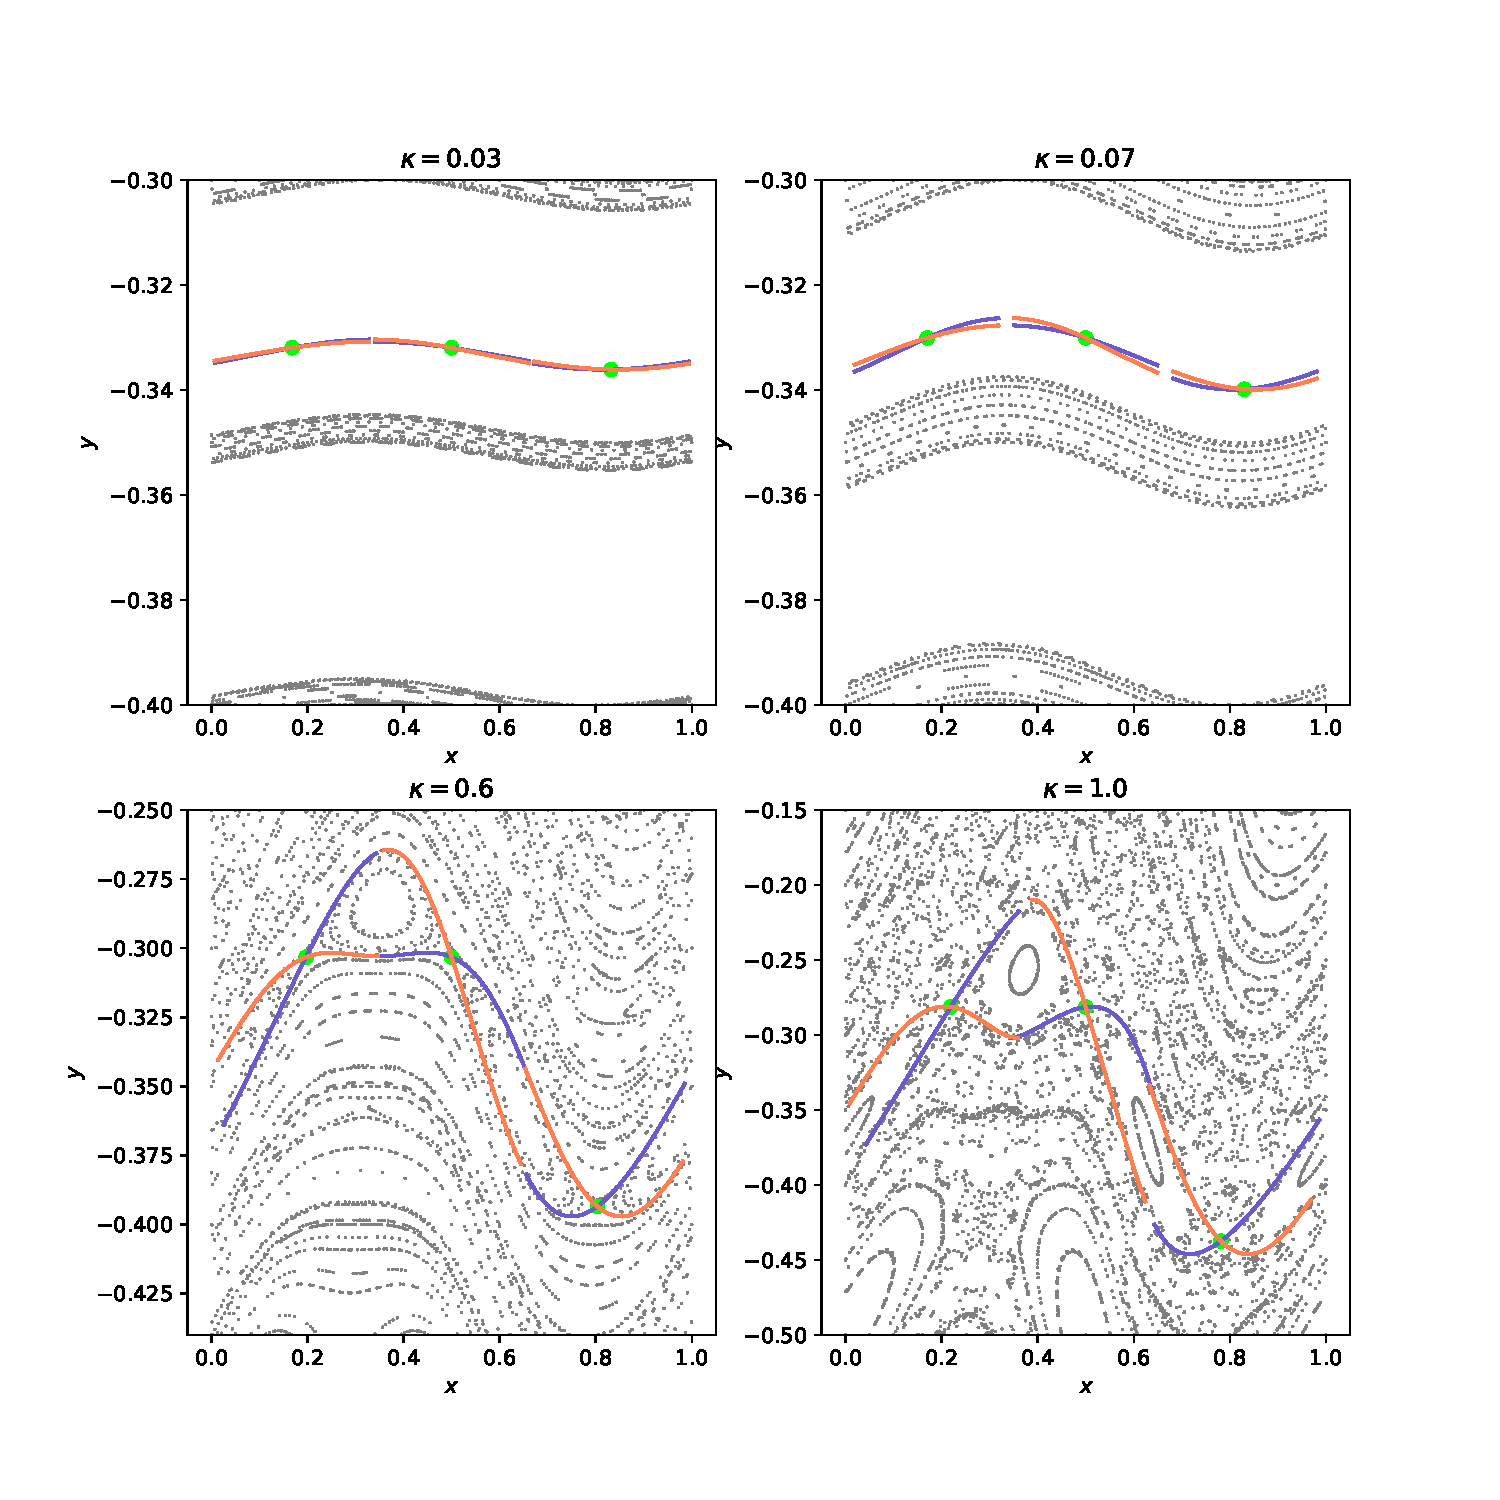
\includegraphics[scale=0.7]{variedadesestandarperiodo3}
	\caption{Variedades invariantes asociadas a una \'orbita de periodo 3 en el mapeo est\'andar con diferentes valores de $\kappa$.}
	\label{variedadesestandarperiodo3}
\end{figure}
\begin{figure}
	\centering
	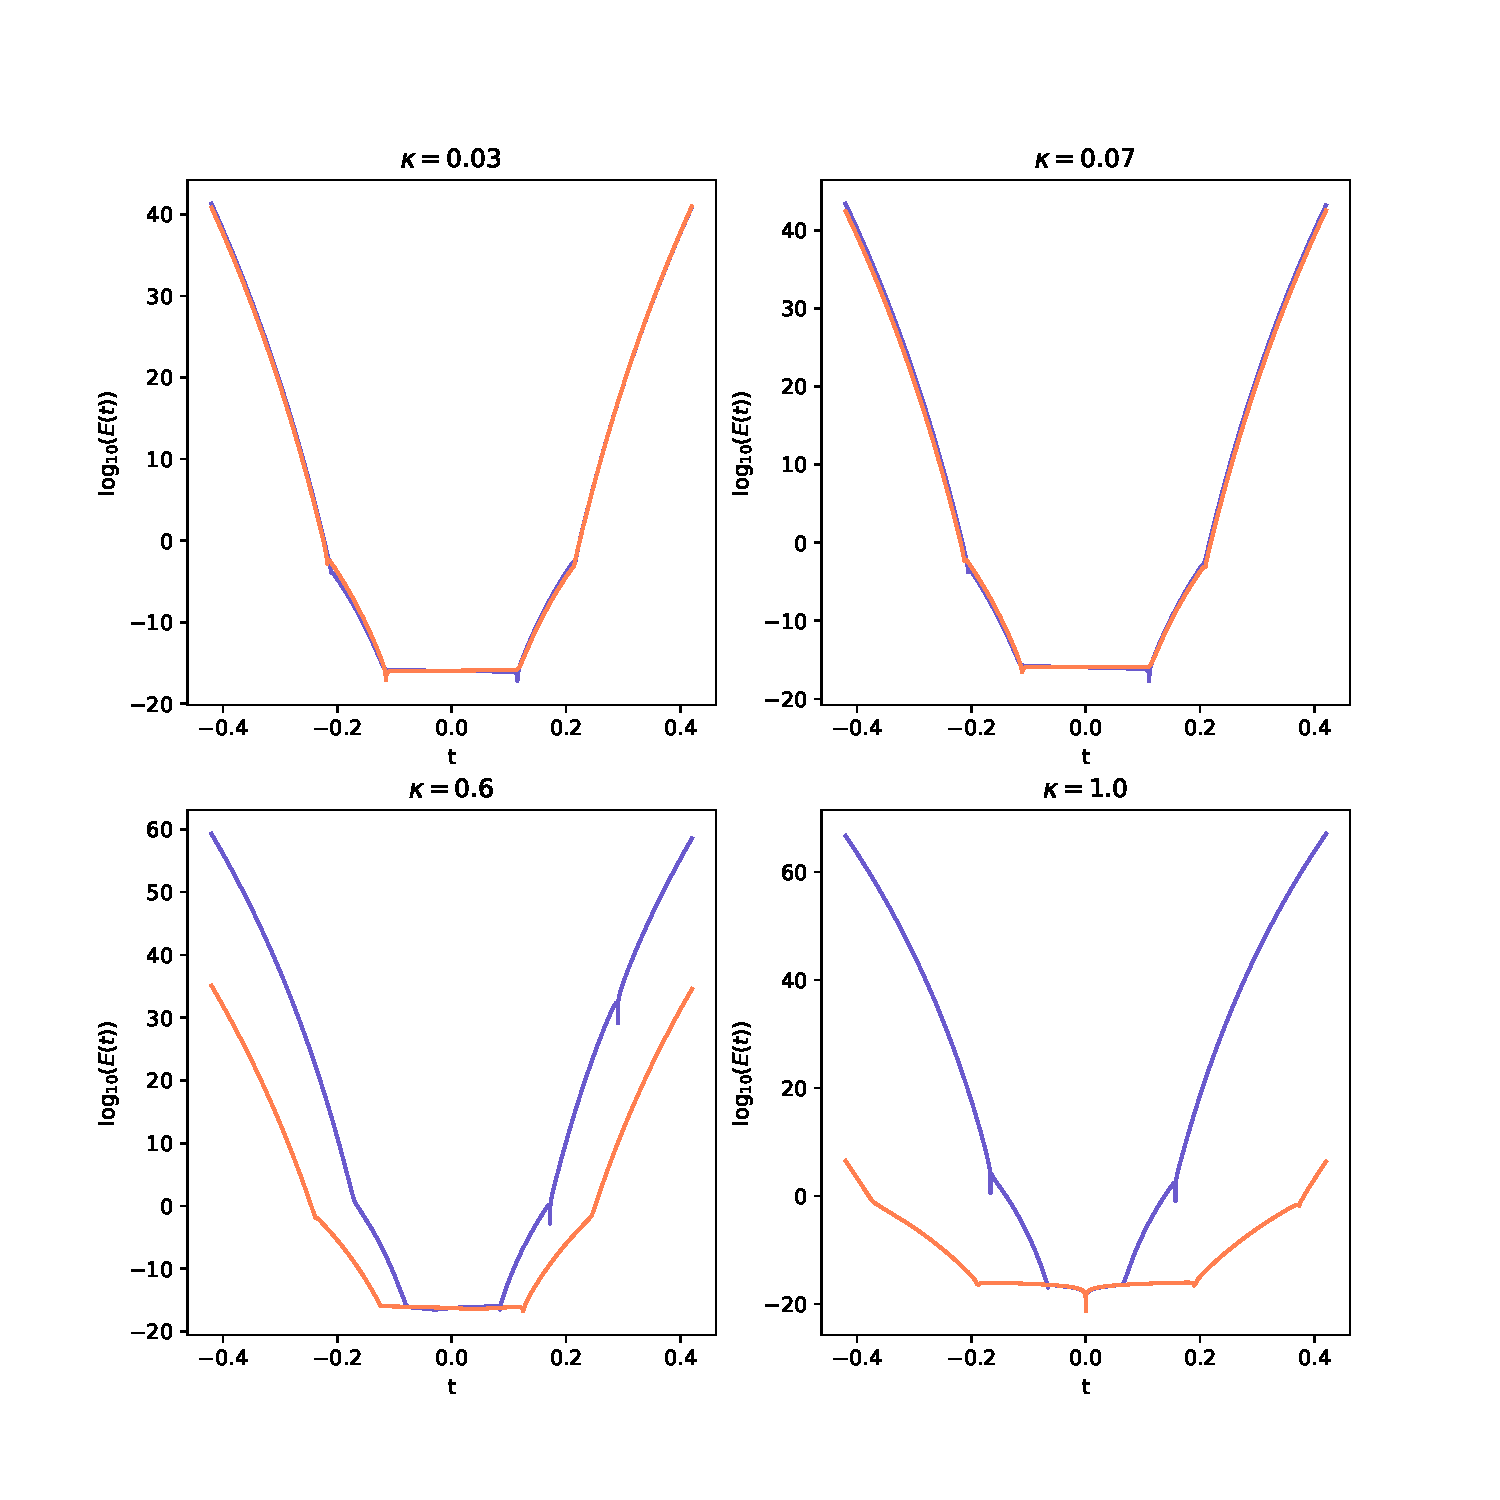
\includegraphics[scale=0.7]{erroresvariedadesestandarperiodo3}
	\caption{Errores asociados al c\'aculo de las variedades invariantes de la figura \ref{variedadesestandarperiodo3}. }
	\label{erroresvariedadesperiodo3}
\end{figure}
\begin{figure}
	\centering
	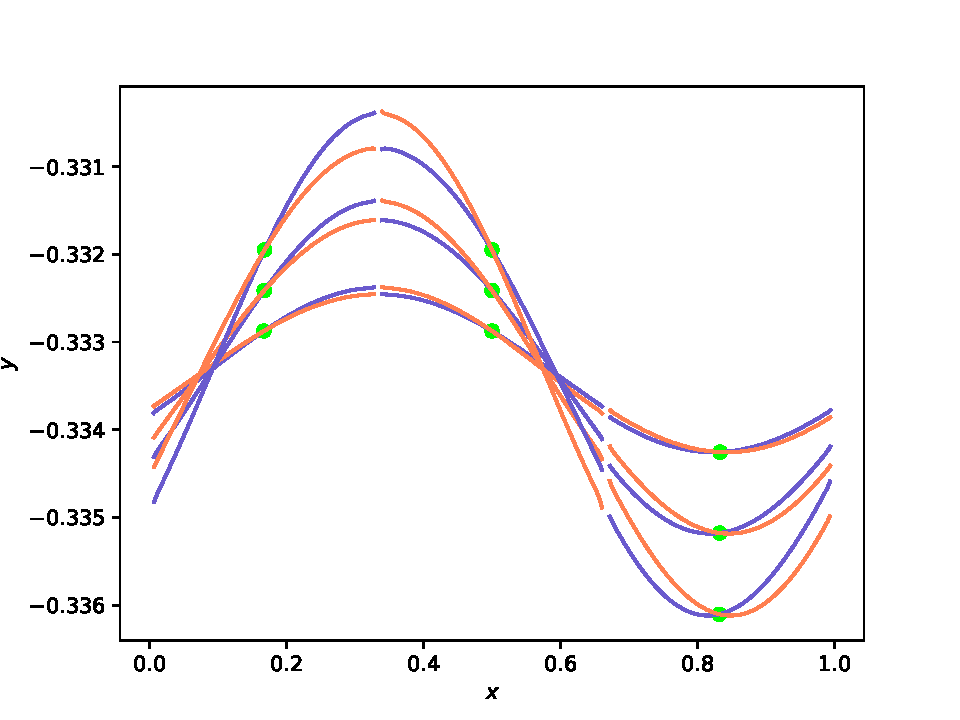
\includegraphics[scale=0.7]{variedadesestperiodo3kvar}
	\caption{Variedades asociadas a una \'orbita de periodo tres para el mapeo est\'andar con valores de $\kappa = [0.01,0.02,0.03]$. }
	\label{vairedadesperiodo3kvariable}
\end{figure}





